% Define the subtitle of the page
\title{Delving In}

% Begin the content of the page
\subsection{Delving In}

Edward enables black box inference for probability models. Its design reflects
the building blocks for inference and model criticism. Here we describe the
motivation behind Edward's design and specify its internal workings.

Edward is named after the innovative statistician
\href{https://en.wikipedia.org/wiki/George_E._P._Box}{George Edward
Pelham Box}. Edward follows Box's philosophy of statistics and machine
learning.

First gather data from a real-world process. Then cycle through Box's
loop:

\begin{enumerate}
\item Build a probabilistic model of the process
\item Reason about the process given model and data
\item Criticize the model, revise and repeat
\end{enumerate}

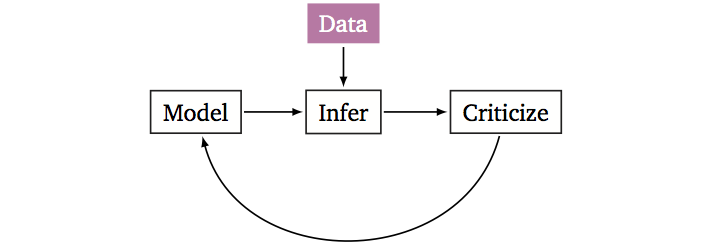
\includegraphics{images/model_infer_criticize.png}

Here's a toy example. A child flips a coin ten times, with the data of
outcomes being \texttt{{[}0,\ 1,\ 0,\ 0,\ 0,\ 0,\ 0,\ 0,\ 0,\ 1{]}}. We
are interested in the probability that the coin lands heads. First,
build a model: assume the coin flips are independent and land heads with
the same probability. Second, reason about the process: use an algorithm
to reason about the model given data. Third, criticize the model: analyze
whether the model captures the real-world process of coin flips. If it
doesn't, then revise the model and repeat.

This process defines the design of Edward. Four primary objects enable the
above analysis.

\subsubsection{Data}

A data object contains measurements. It is a Python dictionary,
typically comprised of strings naming a data object and NumPy arrays
representing their values. For example,

\begin{lstlisting}[language=Python]
my_data = {'x': np.array([0, 1, 0, 0, 0, 0, 0, 0, 0, 1])}
\end{lstlisting}

Data objects can also have their values be TensorFlow tensors in order
to deal with settings such as when the data does not fit in memory.
For more details see the \href{#}{data API}.

\subsubsection{Models}\label{models}

There are two types of model objects in Edward:
\begin{enumerate}
\item Probability models of data, $p(x,z)$
\item Variational models of latent variables $q(z\;;\;\lambda)$
\end{enumerate}

\textbf{Probability Models.}
Edward supports probability models specified in TensorFlow, Python, PyMC3,
or Stan. A probability model has the following structure.
\begin{lstlisting}[language=Python]
import edward as ed
import tensorflow as tf

class probability_model():
    def __init__(...):
        ...
        self.n_vars = ...

    def log_prob(self, xs, zs):
        log_prior = ...
        log_likelihood = ...
        return log_prior + log_likelihood

my_model = probability_model(...)
\end{lstlisting}
The field \texttt{n\_vars} denotes the number of latent variables in the
probability model. For example, a model with a Gaussian likelihood with latent
mean and variance would have \texttt{n\_vars=2*N} latent variables for
\texttt{N} observations.

The method \texttt{log_prob(xs, zs)} calculates the log probability of
the joint density $\log p(x,z)$. Here \texttt{xs} contains the data
and \texttt{zs} are the latent variables. \texttt{xs} can be a single
data point or a batch, and analogously, \texttt{zs} can be a single set or
multiple sets of latent variables.

This describes the probability model, which is a joint distribution of
data $x$ and latent variables $z$. Given a model and data, we aim to
reason about $z$: the model's hidden patterns conditioned on the data. The
posterior distribution $p(z \mid x)$ captures our reasoning: its mean
describes our best guess of the hidden patterns, and its variance
describes the uncertainty around our best guess.

\textbf{Variational Models.}
Edward uses variational inference to approximate the posterior. To
this end, Edward has a \texttt{Variational} class and a library of
\texttt{Distribution} objects. Variational models combine these
using the \texttt{add()} syntax.

For example, to specify this variational model (e.g.~for a Gaussian mixture)
\begin{align*}
  q(z \;;\; \lambda)
  &=
  \text{Dirichlet}(z_\pi)
  \times
  \mathcal{N}(z_\mu)
  \times
  \text{InvGamma}(z_\sigma)
\end{align*}
we would write
\begin{lstlisting}[language=Python]
from edward.models import Variational, Dirichlet, Normal, InvGamma

my_variational = Variational()
my_variational.add(Dirichlet(K))
my_variational.add(Normal(K*D))
my_variational.add(InvGamma(K*D))
\end{lstlisting}
Ordering matters: variational models must match the same ordering as latent
variables accessed in \texttt{probability_model.log_prob(xs, zs)}.

\subsubsection{Inference}\label{inference}

Edward implements a variety of inference methods. Current techniques
leverage variational inference, which seeks to match the variational model
$q(z \;;\; \lambda)$ to the posterior of the probability model
$p(z \mid x)$.

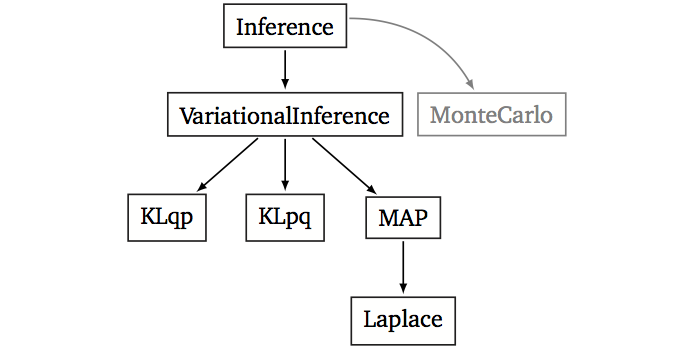
\includegraphics{images/inference_structure.png}
[in caption-style.] Dependency graph of inference methods. Each
node is a class in Edward and arrows represent class inheritance.

Each algorithm minimizes a different loss function between the variational model
and the posterior. Algorithms derived from \texttt{VariationalInference}
take as input a probability model, a variational model, and data.

For example, to minimize the Kullback-Leibler divergence
\begin{align*}
  \text{KL}(p(z \mid x) \;\|\; q(z \;;\; \lambda))
\end{align*}
we would write
\begin{lstlisting}[language=Python]
inference = ed.KLpq(my_model, my_variational, my_data)
inference.run(n_iter=500, n_minibatch=5)
\end{lstlisting}
This runs the \texttt{KLpq} minimization algorithm for \texttt{500} iterations,
using a batch of \texttt{5} data points per iteration.

Edward offers many inference methods; they are best explored through
\href{tutorials.html}{tutorials}.

\subsubsection{Criticism}\label{criticism}

Criticizing models and their inference is a crucial step in analysis.
Following
falsificationists such as Popper and Box, we can never validate
whether a model is true---no model will be true in practice---but we
can seek to uncover where the model goes wrong. Criticism can
help justify the model fit as an approximation or point to good directions
for looping back and revising the model.

To this end, Edward provides a \texttt{criticisms} module that implements:
\begin{enumerate}
  \item posterior predictive checks
  \item metric-based evaluations (e.g.~mean squared error, binary accuracy)
\end{enumerate}

See the \href{tutorials.html}{tutorials} for how to introduce criticism into
your modeling workflow.

\subsubsection{References}\label{references}

\begin{itemize}
\item
  Box, G.E.P. (1976). Science and Statistics. Journal of the American
  Statistical Association, 71(356), 791–799
\item
  Box, G.E.P. (1980). Sampling and Bayes' inference in scientific modelling and
  robustness. Journal of the Royal Statistical Society. Series A. 143(4), 383–430.
\item
  Gelman, A., Meng, X.-L., \& Stern, H. (1996). Posterior predictive assessment
  of model fitness via realized discrepancies. Statistica Sinica.
\item
  David M Blei. (2014). Build, compute, critique, repeat: Data analysis with
  latent variable models. Annual Review of Statistics, 1:203-232
\end{itemize}
